\documentclass{standalone}
\usepackage{graphicx}	
\usepackage{amssymb, amsmath}
\usepackage{color}

\usepackage{tikz}
\usetikzlibrary{intersections, backgrounds}
\usepackage{pgfmath}

\definecolor{light}{RGB}{220, 188, 188}
\definecolor{mid}{RGB}{185, 124, 124}
\definecolor{dark}{RGB}{143, 39, 39}
\definecolor{highlight}{RGB}{180, 31, 180}
\definecolor{gray10}{gray}{0.1}
\definecolor{gray20}{gray}{0.2}
\definecolor{gray30}{gray}{0.3}
\definecolor{gray40}{gray}{0.4}
\definecolor{gray60}{gray}{0.6}
\definecolor{gray70}{gray}{0.7}
\definecolor{gray80}{gray}{0.8}
\definecolor{gray90}{gray}{0.9}
\definecolor{gray95}{gray}{0.95}

\newcommand*{\offset}{0.025}

\begin{document}

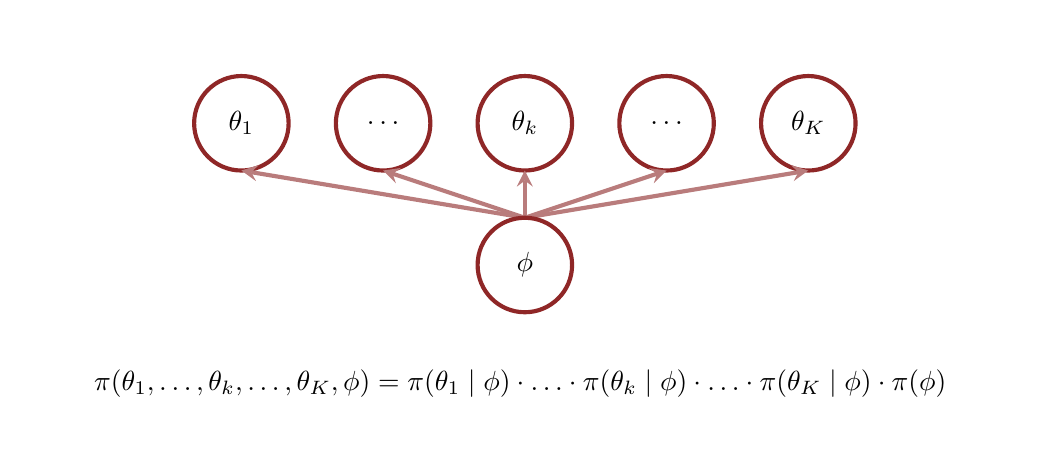
\begin{tikzpicture}[scale=0.3, thick]

\pgfmathsetmacro{\r}{2}

\pgfmathsetmacro{\dx}{0}
\pgfmathsetmacro{\dy}{0}

\draw[white] (-21 + \dx, -10 + \dy) rectangle (21 + \dx, 7 + \dy);

\node[align=center] at (0 + \dx, -8 + \dy) 
{ $ \pi(\theta_{1}, \ldots, \theta_{k}, \ldots, \theta_{K}, \phi) 
    = \pi(\theta_{1} \mid \phi) \cdot \ldots \cdot \pi(\theta_{k} \mid \phi) 
      \cdot \ldots \cdot \pi(\theta_{K} \mid \phi) \cdot \pi(\phi) $ };

\filldraw[fill=white, draw=dark, line width=1.5] (-12 + \dx, 3 + \dy) circle (\r)
node[color=black] { $\theta_{1}$ };

\filldraw[fill=white, draw=dark, line width=1.5] (-6 + \dx, 3 + \dy) circle (\r)
node[color=black] { $\ldots$ };

\filldraw[fill=white, draw=dark, line width=1.5] (0 + \dx, 3 + \dy) circle (\r)
node[color=black] { $\theta_{k}$ };

\filldraw[fill=white, draw=dark, line width=1.5] (6 + \dx, 3 + \dy) circle (\r)
node[color=black] { $\ldots$ };

\filldraw[fill=white, draw=dark, line width=1.5] (12 + \dx, 3 + \dy) circle (\r)
node[color=black] { $\theta_{K}$ };

\draw[->, >=stealth, color=mid, line width=1.5] (0 + \dx, -3 + \r + \dy) -- (-12 + \dx, 3 - \r + \dy);
\draw[->, >=stealth, color=mid, line width=1.5] (0 + \dx, -3 + \r + \dy) -- (-6 + \dx, 3 - \r + \dy);
\draw[->, >=stealth, color=mid, line width=1.5] (0 + \dx, -3 + \r + \dy) -- (0 + \dx, 3 - \r + \dy);
\draw[->, >=stealth, color=mid, line width=1.5] (0 + \dx, -3 + \r + \dy) -- (6 + \dx, 3 - \r + \dy);
\draw[->, >=stealth, color=mid, line width=1.5] (0 + \dx, -3 + \r + \dy) -- (12 + \dx, 3 - \r + \dy);

\filldraw[fill=white, draw=dark, line width=1.5] (0 + \dx, -3 + \dy) circle (\r)
node[color=black] { $\phi$ };

\end{tikzpicture}

\end{document}  